\section{Construction du profiling}

L'objectif de cette partie était d'analyser et d'interpréter les traces de sortie d'exécution du code à compiler.\\

Nous avons donc développé un parseur LEX et YACC capable d'analyser les traces statiques et dynamiques issues du code instrumenté.\\

\subsection{Parsing LEX et YACC}

Les traces issues de l'instrumentation dynamique se présentent sous la forme suivante:
\begin{verbatim}
Appel X à la fonction main entrée cycle WW sortie cycle YY
Appel X à la fonction f1 entrée cycle WW sortie cycle YY
Appel X à la fonction f2 entrée cycle WW sortie cycle YY
\end{verbatim}

La grammaire reconnaissant les traces dynamiques est la suivante:
\begin{verbatim}
CALL FUNCTION NAME ENTERCYCLE NUMERIC EXITCYCLE NUMERIC RETLINE
\end{verbatim}

ENTERCYCLE et EXITCYCLE correspondent aux temps de début et de fin d'exécution d'une fonction.

\subsection{Profilage exclusif}

Le profilage issu du fichier de trace est inclusif, dans le sens où le temps total d'exécution d'une fonction inclut les temps d'exécution des fonctions appelées depuis la fonction parente.\\
L'analyse du fichier de traces se propose de produire un profilage exclusif, c'est-à-dire le temps d'exécution d'une fonction seule.\\

Pour pouvoir construire le profilage exclusif des fonctions, nous avions besoin de connaître les imbrications entre elles, et nous avons opté pour une construction sous forme d'arbres n-aires, où chaque noeud représente une fonction.\\

Pour celà, nous avons utilisé une représentation sous forme d'arbres n-aires.\\
La première fonction analysée constitue la racine de l'arbre (il s'agira du point d'entrée main() par exemple). Ensuite, pour chaque nouvelle fonction reconnue par l'analyseur, celui-ci créé un noeud qui est comparé aux noeuds précédents, en fonction des temps d'entrée et de sortie de la fonction.\\
Le noeud précédent le plus récent contenant une mesure d'entrée inférieure et une mesure de sortie supérieure au noeud dernièrement créé devient le parent de celui-ci. Le temps exclusif de la fonction parente est alors calculée en soustrayant son temps inclusif par le temps inclusif de la fonction enfant.\\

\begin{center}
  \begin{dot2tex}[neato,mathmode]
    digraph {
       label="main->exclusive time = main->inclusive time - func1->inclusive time"
      "main" -> "func1" 
      "func1" [style="fill=red!80"]
    }
  \end{dot2tex}
  \captionof{figure}{Add a first node}
\end{center}

Si un autre noeud ayant le même parent est ajouté, alors on soustrait à nouveau le temps exclusif du parent par le temps inclusif du nouveau noeud ajouté.\\

\begin{center}
  \begin{dot2tex}[neato,mathmode]
    digraph {
   label="main->exclusive time = main->exclusive time - func2->inclusive time"
   "main" -> "func1" 
   "main" -> "func2"
   "func2" [style="fill=red!80"]
    }
  \end{dot2tex}
  \captionof{figure}{Add a second node}
\end{center}

L'opération est répétée jusqu'à la fin de l'analyse du fichier de traces, jusqu'à obtenir le temps exclusif de toutes les fonctions.\\

\subsection{Gestion des instances}

L'un des objectifs du profiling est de pouvoir comparer les temps d'exécution de différentes instances d'une fonction.\\ 
Jusqu'à maintenant, tous les appels d'une même fonction sont chacune représentés par un noeud unique (on rajoute un noeud à chaque ligne lue).\\

\begin{center}
	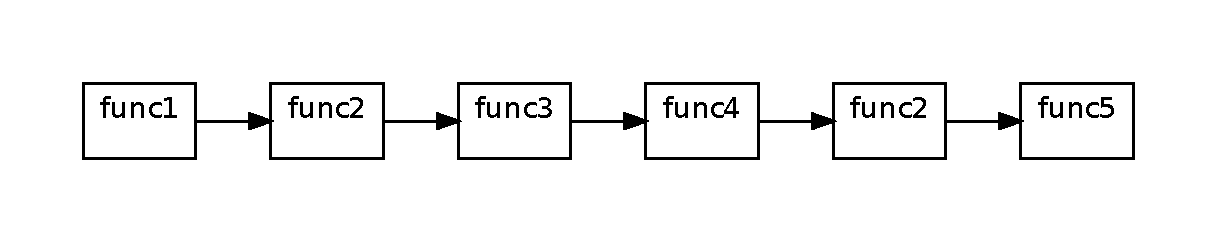
\includegraphics[scale=0.50]{images/liste1}
	\captionof{figure}{Nodes list}
\end{center}

Nous avons avant tout besoin de détecter les fonctions redondantes du fichier d'entrée, puis les considérer comme des instances différentes d'une même fonction.
Pour établir le nombre d'instances par fonction, l'analyseur reparcourt la liste des noeuds, identifie celles ayant le même nom, puis les stocke dans une structure, en renseignant le nombre d'instances.\\

\begin{center}
	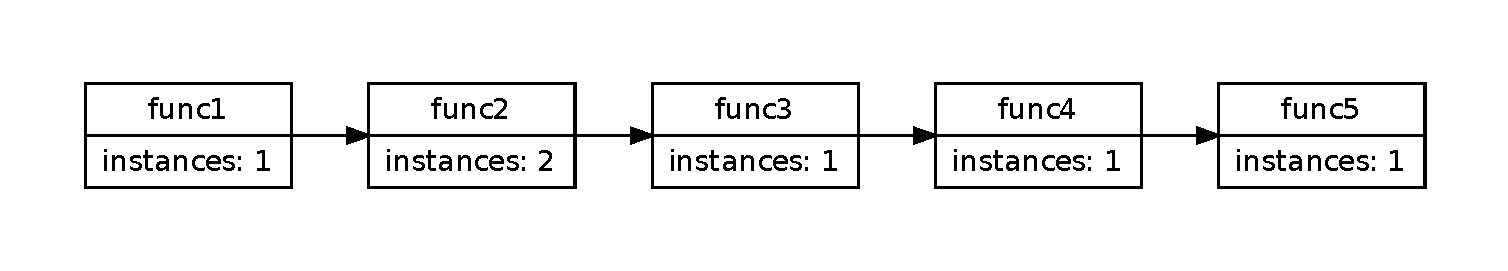
\includegraphics[scale=0.50]{images/ListIntances}
	\captionof{figure}{Nodes list with instances}
\end{center}

Les données recueillies sont ainsi sérialisées dans un fichier de sortie, puis interprétées en vue de produire un diagramme gnuplot \\

\subsection{Corrélation des instrumentations statique et dynamique}

La seconde partie du profiler consiste à corréler les données statiques et dynamiques d'une fonction, à savoir confronter le temps d'exécution et le nombre de load/store. Dans cette optique, nous avons construit une grammaire lui permettant de reconnaître les données issues de l'instrumentation statique:

\begin{verbatim}
FUNCTION NAME RETLINE
NUMERIC LOAD RETLINE
NUMERIC MUL NUMERIC LOAD RETLINE
NUMERIC STORE RETLINE
NUMERIC MUL NUMERIC STORE RETLINE
\end{verbatim}

Une fois les données statiques lues, on peut calculer le nombre de load et de store par fonction, puis, en parcourant la liste des fonctions déjà stockées, faire correspondre le nombre de load/store aux données dynamiques de la fonction précédemment analysée.\\

Une piste envisagée (qui a été implémentée), était de calculer une estimation de la latence d'un load et d'un store. Cette opération revenait à résoudre un système d'équations à deux inconnues (load et store), dont le résultat serait le temps d'exécution de la fonction concernée.\\
On résout le système en prenant en entrée un couple de fonctions, ce qui se traduit par:
\begin{verbatim}
load1*FacteurLoad1 + store1*FacteurStore1 = TempsFonction1
load2*FacteurLoad2 + store2*FacteurStore2 = TempsFonction2
\end{verbatim}
Système qui a été résolu en utilisant la méthode de Cramer.\\

L'opération a été répétée sur toutes les fonctions (en conservant la même fonction comme première équation), afin de calculer une moyenne sur les load/store.
Cependant, cette piste a été écartée en raison de la volatilité des mesures d'accès mémoire.\\ 

\subsection{Graphe d'appel}

Enfin, le profiler propose la génération d'un graphe d'appel des fonctions, à l'aide d'un parcours préfixé de l'arbre n-aire construit. Il produit en sortie un fichier compréhensible par l'outil dot.

\begin{center}
	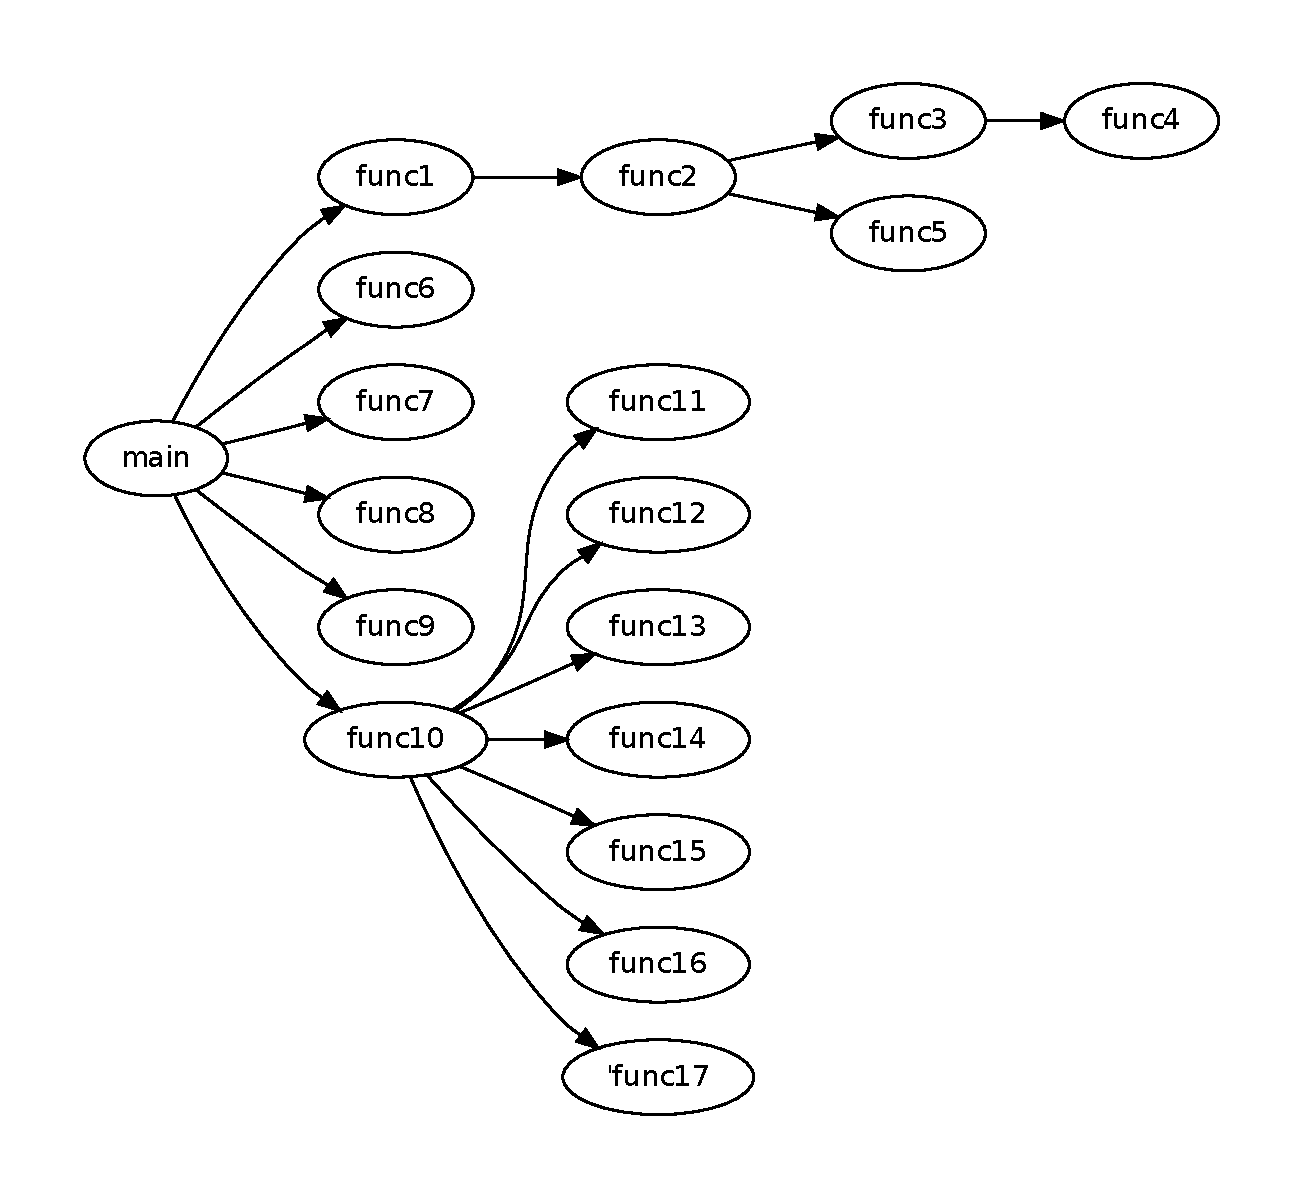
\includegraphics[scale=0.50]{images/CallGraph}
	\captionof{figure}{Functions Call Graph}
\end{center}


